\section*{Results}

\begin{figure*}[h!]
%\begin{center}
%\begin{subfigure}[t]{\textwidth}
\centering
%\caption{}
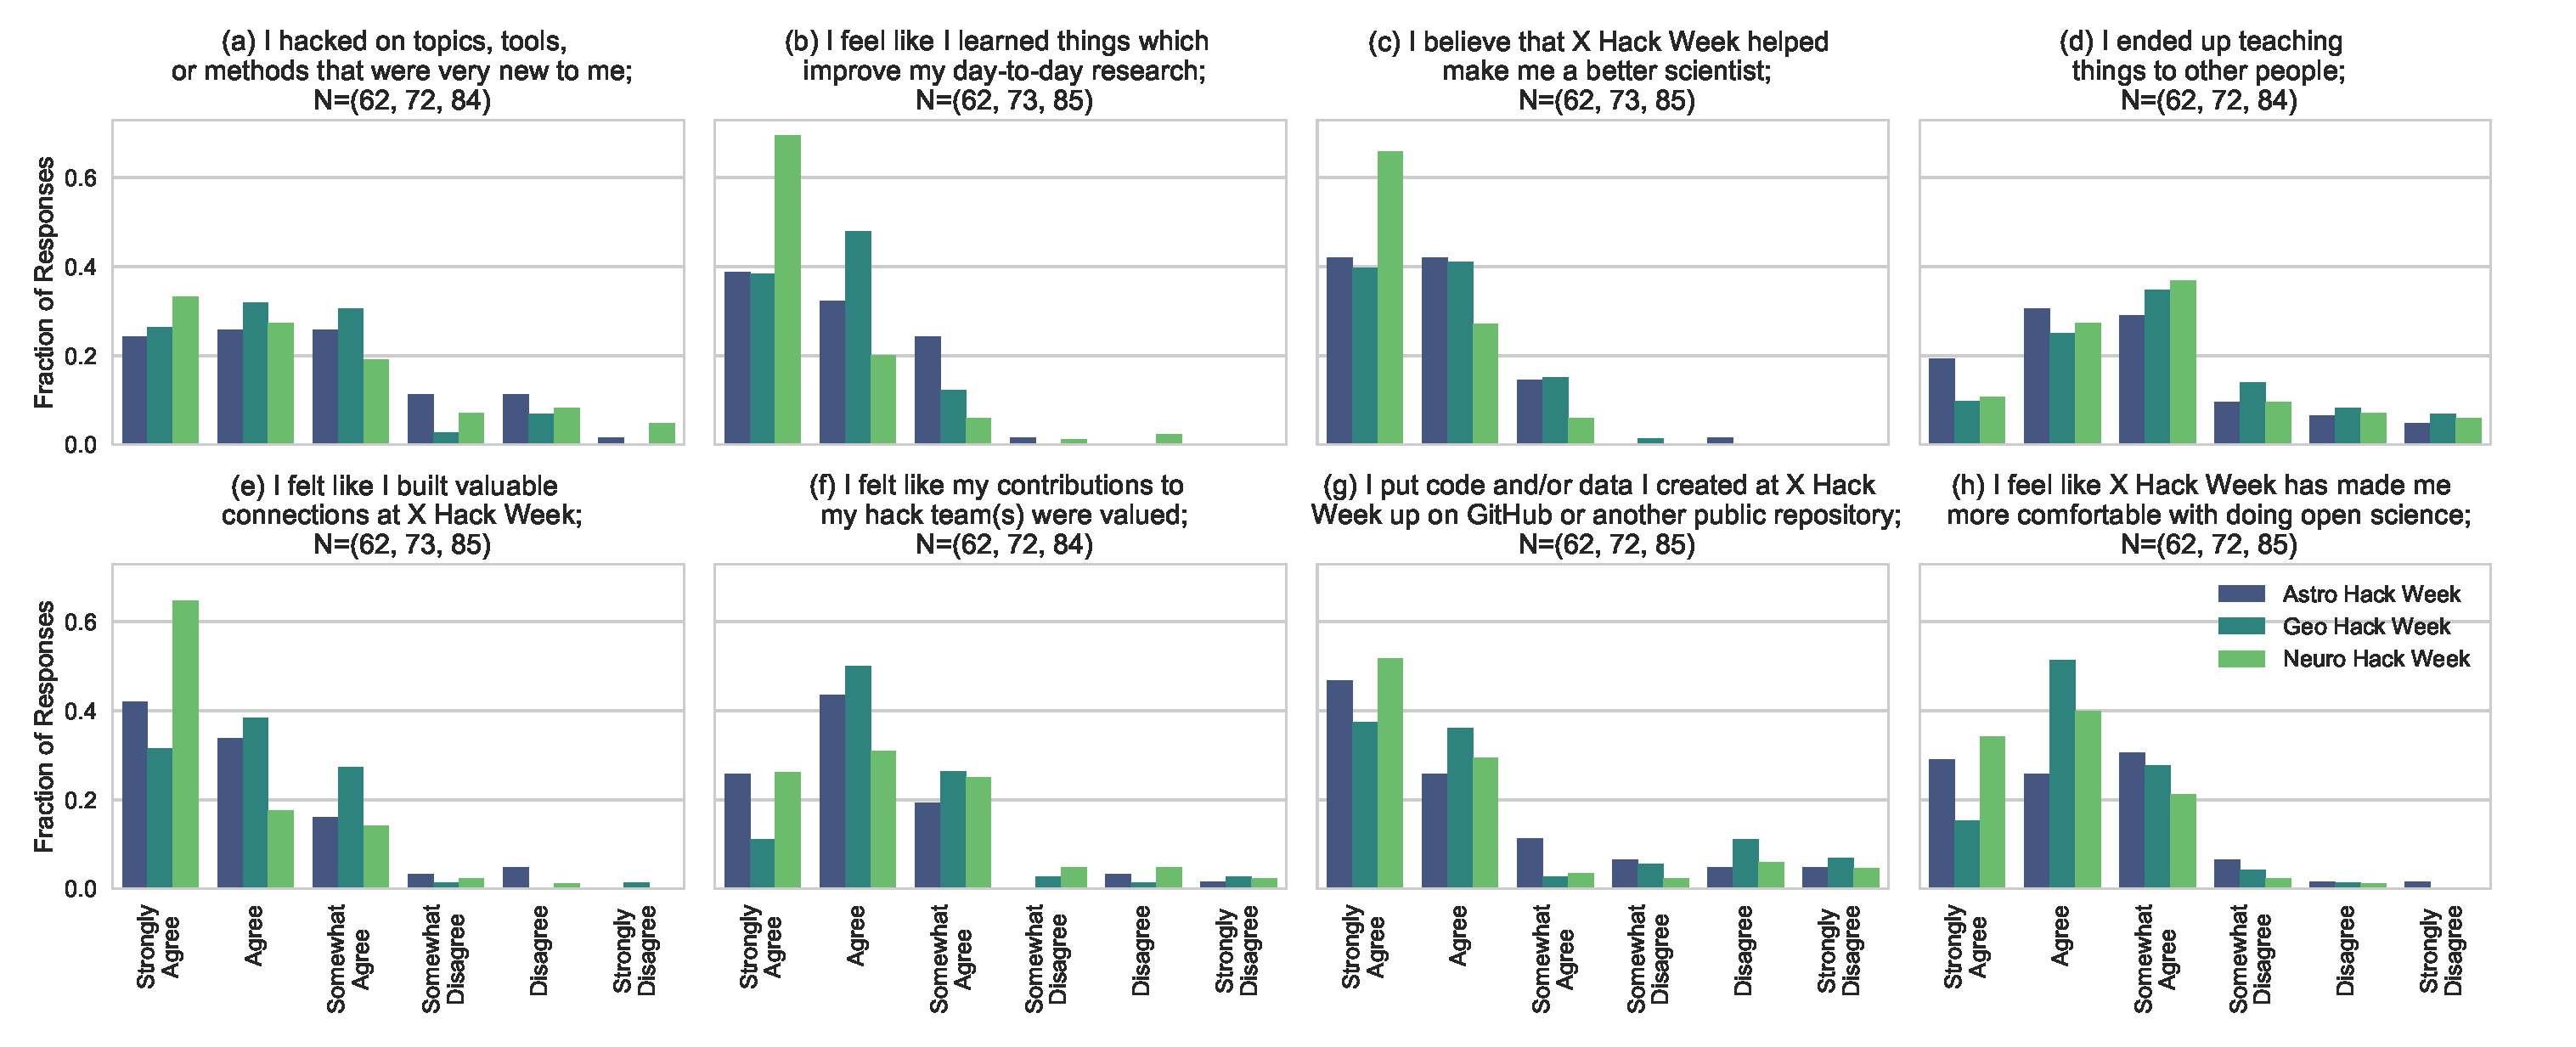
\includegraphics[width=\textwidth]{f2.eps}
%\end{subfigure}
\caption{Post-workshop surveys from three hack weeks: participants in the 2016 astro-, geo- and neuro- hack weeks responded to questions assessing their experiences. Response rates are reported in the panel titles for AHW, GHW and NHW, respectively. We report here about results in three different domains: the development of technical skills (a -- c), collaboration and teaching (d -- f), and shifts in attitudes towards reproducibility and open science (g, h).}
\label{fig:survey}
%\end{center}
\end{figure*}

\begin{table*}
%\begin{table*}[hbtp]
%\renewcommand{\arraystretch}{1.3}
\footnotesize
\caption{}
\begin{threeparttable} 
\begin{tabularx}{18cm}{p{3.4cm}p{0.3cm}p{0.33cm}p{0.33cm}p{0.33cm}p{0.33cm}p{0.33cm}p{0.33cm}p{0.33cm}p{0.33cm}p{0.33cm}p{0.33cm}p{0.33cm}p{0.33cm}p{0.33cm}p{0.33cm}p{0.33cm}p{0.33cm}p{0.33cm}}
\toprule
\textbf{Question} & \multicolumn{6}{c}{\textbf{Astro Hack Week}} & \multicolumn{6}{c}{\textbf{GeoHackWeek}} & \multicolumn{6}{c}{\textbf{NeuroHackWeek}} \\ \midrule
 & $N$ & $\mathrm{dof}_{\chi^2}^\emph{a}$ & $\chi^2$ & $p$ & $\mathrm{dof}_{\phi_c}^\emph{b}$ & $\phi_c$ & $N$ & $\mathrm{dof}_{\chi^2}^\emph{a}$ & $\chi^2$ & $p$ & $\mathrm{dof}_{\phi_c}^\emph{b}$ & $\phi_c$ & $N$ & $\mathrm{dof}_{\chi^2}^\emph{a}$ & $\chi^2$ & $p$ & $\mathrm{dof}_{\phi_c}^\emph{b}$ & $\phi_c$ \\ \midrule
\multicolumn{16}{l}{\textbf{Comparison with career stage (early-career stage; faculty and research scientists; other)}}  \\ \midrule
New topics, tools, methods (a) & 61 & 10 & 5.64 & 0.85 & 1.93 & 0 & 36 & 6 & 2.51 & 0.87 & 1.88 & 0 & 41& 10 & 15.53 & 0.15 & 1.9 & 0.23 \\
Improvement of research (b) & 61 & 6 &  9.89 & 0.13 & 1.93 & 0.18 & 35 & 4 & 12.41 & 0.02 & 1.88 & 0.35 & 40 & 6 & 7.42 & 0.28 & 1.90 & 0.13 \\
Better science (c) & 59 & 6 & 3.79 & 0.70 & 1.93 & 0 & 35 & 4 & 10.61 & 0.03 & 1.88 & 0.31 & 40 & 4 &  5.06 & 0.29 & 1.90 & 0.11\\ 
Teaching (d) & 61 & 10 & 13.65 & 0.19 & 1.93 & 0.17 & 36 & 10 & 13.68 & 0.19 & 1.88 & 0.22 & 40 & 10 & 6.90 & 0.74 & 1.90 & 0 \\ \midrule
\multicolumn{16}{l}{\textbf{Gender Identity (non-minority; minority)}} \\ \midrule
Improvement of research (b) & 60 & 3 & 2.08 & 0.56 & 0.98 & 0 & 35 & 2 & 5.26 & 0.07 & 0.97 & 0.30 & 40 & 3 & 7.62 & 0.05 & 0.97 & 0.34\\
Teaching (d) & 61 & 5 & 7.30 & 0.20 & 0.98 & 0.19 & 36 & 5 & 12.71 & 0.26 & 0.97 & 0.46 & 40 &5 & 3.17 & 0.67 & 0.97 & 0 \\
Connection building (e) & 61 & 4 & 3.70 & 0.45 & 0.98 & 0 & 36 & 3 & 5.89 & 0.12 & 0.97 & 0.28 & 41 & 3 & 4.42 & 0.22 & 0.98 & 0.18\\
Valued contributions (f) & 57 & 4 & 5.98 & 0.20 & 0.98 & 0.18 & 34 & 5 & 9.46 & 0.09 & 0.97 & 0.36 & 38 & 5 & 6.75 & 0.34 & 0.97 & 0.21 \\ \midrule
\multicolumn{16}{l}{\textbf{Racial/ethnic Identity (white; non-white)}} \\ \midrule
Improvement of research (b)  & 59 & 3 & 0.97 & 0.81 & 0.98 & 0 & 34 &2 & 0.01 & 0.99 & 0.97 & 0 & 39 & 3 & 2.79 & 0.43 & 0.97 & 0 \\
Teaching (d) & 61 & 5 & 5.63 & 0.34 & 0.98 & 0.09 & 34 & 4 & 1.29 & 0.86 & 0.97 & 0 & 39 & 5 & 3.06 & 0.69 & 0.97 & 0 \\
Connection building (e) & 61 & 4 & 1.64 & 0.80 & 0.98 & 0 & 34 & 3 & 8.42 & 0.04 & 0.97 & 0.40 & 40 & 3 & 3.49 & 0.32 & 0.97 & 0.10 \\
Valued contributions (f) & 58 & 4 & 13.14 & 0.01 & 0.98 & 0.40 & 32 & 5 & 2.49 & 0.78 & 0.96 & 0 & 37 & 5 & 4.05 & 0.54 & 0.97 & 0 \\ 
\bottomrule
\end{tabularx}
   \begin{tablenotes}
      \item{Respondents to a post-event evaluation survey indicate their level of agreement on a six-point Likert-type scale to a range of statements (letters correspond to panels in Figure \ref{fig:survey}). Results are for hack weeks held in 2016 and 2017 for AHW and in 2016 for GHW and NHW, respectively. The number of respondents for each question is included in the table above. Additional figures showing the distributions of responses for each question are available in the SM, Section 6.}
      \item[\emph{a}]{While the range of Likert items was the same for every question, the degrees of freedom for $\chi^2$ and Cram\'{e}r's V may differ depending on the number of items with non-zero responses, and the number of non-zero items in the independent variable.}
      \item[\emph{b}]{The degrees of freedom for Cram\'{e}r's V corrected according to~\citep{bergsma2013}}
\end{tablenotes}

\end{threeparttable}
\label{tab:survey}
%\end{table*}
\end{table*}



Measuring the success of a hack week objectively is complicated by the variety of goals that a hack week might have (see above). 
Additionally, the participant-driven format facilitates knowledge transfer and collaborations in sometimes surprising ways that escape traditional measures of success.

One key metric is the number of publications that result from hack week projects, but this is a fairly narrow definition of success, in line with standard academic performance indicators.
Assuming that participants work largely in the open during a hack week, and that most projects have a strong programming component, another indicator of success is the activity of participants in terms of code written and committed to a public code repository.
Still, these measures ignore learning, community-building as well as networking outcomes, which can be assessed through post-workshop surveys.
Here, we have taken an approach that combines these metrics: we start with survey results, and anecdotally report about publications and projects generated (see the following section).

Focusing on the outcomes of astro-, geo- and neuro- hack weeks (AHW, GHW, NHW, respectively) from 2016 and 2017, we find that most participants self-report successful learning outcomes (AHW: 76\%, GHW: 89\%, NHW: 79\% for responses ``somewhat agree'', ``agree'' and ``strongly agree''; Figure \ref{fig:survey}, (a)).
The overwhelming majority of respondents at the hack weeks ($>95\%$ for all three events) believed that they learned things that improve their day-to-day research, and that attendance has made them a better scientist (Figure \ref{fig:survey}, (b, c)).
%More specifically, we compared learning outcomes in data visualization (the only topic explicitly shared between all three hack weeks; Figure \ref{fig:survey}, (d, e). We asked participants to subjectively rate their knowledge before the hack week, and find skill levels to be broadly distributed. This is expected, given the goal of diversity during the selection stage. We find that most participants have positive learning outcomes at all three hack weeks for data visualization, but that outcomes vary strongly, as is expected, too, with a group that is this diverse. We also note that there might be systematic effects and biases due to the subjectivity of rating knowledge and learning outcomes.
Because peer learning is a major mode of knowledge transfer at hack weeks, we asked participants whether they taught other participants.
We find that again a majority agrees with this statement to some degree (AHW: 79\%, GHW: 69\%, NHW: 75\%; Figure \ref{fig:survey}, (d)), though responses are not as unequivocal as they are in some of the other categories.
The majority of participants felt that they built valuable connections to other researchers (Figure \ref{fig:survey}, (e)), especially at NHW, where more than 64\% of participants strongly agreed with this statement. 

Given the broad diversity in skills and backgrounds of participants admitted to our hack weeks, a dependence of learning outcomes and teaching on career stage is plausible. At the same time, we suggested earlier in this paper that peer learning is a major mode of knowledge transfer during hack weeks, and that this type of learning takes place at all career stages. We find no strong evidence for a significant difference between early-career researchers and senior participants for any of the three hack weeks for questions regarding learning outcomes of new tools and topics (a), improvements in day-to-day research (b) or overall improvements in science (c) (all statistical results are presented in Table \ref{tab:survey}). Only for GHW we find a weak indication that early-career researchers agree more strongly that the hack week improved their day-to-day research (p=0.02) with a large effect size of $\phi_c = 0.4$ (following~\citep{cohen1988}). 
Similarly, we find no strong indication that late-career researchers self-report a higher level of teaching at hack weeks compared to early-career researchers (d).

One important question regarding hack week outcomes is whether participants from underrepresented groups thrive at these events, or whether their full participation is impeded. Significant differences between minorities and non-minorities, even on a self-reported scale, for questions related to learning outcomes, teaching or network building would indicate that improvements in workshop facilitation and structure may be required to allow participants of all stripes to participate fully.
In Section 4 of the Supplementary Materials, we lay out various strategies we have employed to facilitate participation, empower members of underrepresented groups and mitigate impostor syndrome. Based on our surveys, we find no significant dependence of self-reported learning outcomes on gender identity or race/ethnicity (Table \ref{tab:survey}). Similarly, minority participants with respect to gender identity and race or ethnicity do not significantly differ in their answers with respect to teaching outcomes for any of the hack weeks. Both underrepresented groups similarly feel that they built equally valuable connections at all three hack weeks and generally feel that their contributions to their hack teams were valued. For GHW, there is a weak indication that participants from racial/ethnic minorities respond more positively when asked about building connections (p=0.04) with a medium to large effect size ($\phi_c = 0.4$), while for AHW, responses regarding the value of contributions to hack teams may be spread more widely for participants from racial/ethnic minorities than for Caucasian participants ($p = 0.01; \phi_c = 0.4$). These initial results indicate that future work on how demographics interact with hack week attendance may be fruitful. We note that since we did not include a question about impostor syndrome itself, we cannot draw causal connections between our results and its prevalence. Additionally, our number of respondents is small, and the lack of significant differences may be caused by the small statistical power of our sample.
%It is notable, however, that we find no correlation between the response to this question and career stage for any of the events surveyed here. Participants at all career stages report similar engagement in teaching. This suggests there is some evidence for our hypothesis that compared to e.g.\ a traditional summer school, a hack week is less hierarchical and encourages lateral knowledge transfer between participants at different career stages. However, we note that the sample sizes per category are relatively small, and future work is needed to confirm this hypothesis. We similarly find no correlations with gender identity or race/ethnicity.

We find that the hack weeks have been largely successful at efforts to promote positive attitudes towards reproducibility and open science: at all three events, the majority reports that the hack week has made them more comfortable with open science  (GHW: 97\%; NHW: 95\%; AHW: 72\%, Figure \ref{fig:survey}, (h)). At all three events, more than 85\% of all participants (AHW: 86\%, GHW: 94\%, NHW: 95\%; Figure \ref{fig:survey}, (g)) put code or data created at the hack week into a public repository.
%The overall behaviour hints at how general conventions and attitudes differ in different fields.
%Astronomy shows the largest degree of openness toward open science, whereas our results indicate that open science is still fairly uncommon in the geosciences, with neuroscience falling in between.
%Similar attitudes are reflected when asking whether the hack week has made participants more comfortable with open science (Figure \ref{fig:survey}, (j)): again, geoscience shows the large improvement with over 97\% agreeing with this statement to some degree, followed by neuroscience (95\%) and astronomy (72\%).
%Overall, our results indicate that hack weeks are effective at addressing persisting doubts about making research open and reproducible. 
While the focus on open science is not necessarily a required component of a hack week, it aligns naturally with many of the goals and values commonly promoted at hack weeks like open-source software and data sharing. In some fields, especially where ethical issues around data sharing and privacy are relevant, this might not be a desired focus of the hack week, or might be replaced or augmented by a discussion of ethical considerations.

We caution the reader that the survey results should be read only as an indication of the hypotheses we proposed about the use and outcomes of hack weeks, in line with the exploratory nature of the surveys conducted as part of past hack weeks we have organized. The most important independent variable--attendance at the hack week--is something that our current survey design cannot account for. Moreover, self-reported learning outcomes are not an objective measure, because they are likely subject to internal biases of respondents. Future work will include more a more refined survey design as well as attendance versus non-attendance as a control variable.

Because all three events are relatively recent, it is still early to evaluate long-term outcomes, as well as others including publications and collaborations resulting from these events.
There are, however, initial indicators that all hack weeks encouraged long-term engagement with new concepts or tools and that they directly resulted in a number of publications \cite{gullysantiago2015,faria2016,keshavan2017,leonard2017,jordan2017,peterson2017,hahn2017,pricewhelan2017}. For specific examples, see also below.

\subsection*{Examples of Hack Week Outcomes}
\label{sec:outcomes}
\subsubsection*{Example 1: Astro Hack Week}
In 2015, a small team used AHW to found a new software project called Stingray\footnote{https://github.com/StingraySoftware/stingray} with the goal of providing well-tested implementations of time series analysis algorithms often used in X-ray astronomy.
The start of this project was facilitated by the collaborative environment at Astro Hack Week, including expertise in how to start/run open-source projects and role models of successful projects. Astro Hack Week enabled participants to seed a new collaboration around a software project needed by the larger community.
Stingray has since matured into an enduring collaboration within the community with five active maintainers and four Google Summer of Code projects.
\subsubsection*{Example 2: Geo Hack Week}
In 2016, a GHW project team used Google Earth Engine to explore spatial patterns in climate, topography and population data with the goal of mapping the most suitable locations for renewable energy sites in the United States.
The team used machine learning algorithms in conjunction with the powerful hardware resources provided by Google Earth Engine\footnote{\url{http://georgerichardson.net/2017/04/10/searching-for-energy-in-a-random-forest/}}.
George Richardson, one of the project leads, now works for a renewable resource company in Seattle.
\subsubsection*{Example 3: Neuro Hack Week}
Motion of study participants inside of the MRI machine is a major concern in neuroimaging studies.
During NHW 2016 one of the teams focused on a large and openly available data-set of MRI data from children\footnote{ABIDE: \url{http://preprocessed-connectomes-project.org/abide}}.
To test the effect of motion on the results, the team conducted an analysis in which both the number of experimental subjects included, as well as motion cut-off were varied.
%They tested both the split-half reliability of an analysis of brain connectivity, as well as an analysis that used machine learning to distinguish between brains of children with and without autism spectrum disorder.
The team (composed of four researchers from four institutions) continued to work on this project remotely after the end of NHW, and eventually published a paper describing these results in the open access journal Research Ideas and Outcomes \cite{leonard2017}.
